\section{Cortex-M Architecture}

\begin{concept}{Core Architecture Overview}\\
The ARM Cortex-M is a 32-bit processor architecture designed for embedded systems:
\begin{itemize}
  \item Load/store architecture
  \item 32-bit data path
  \item Thumb instruction set
  \item Hardware multiply and optional divide
\end{itemize}
\end{concept}

\begin{definition}{Core Registers}\\
The Cortex-M has 16 core registers, each 32-bit wide:
\begin{itemize}
  \item \textbf{R0-R7}: Low registers - general purpose
  \item \textbf{R8-R12}: High registers - general purpose
  \item \textbf{R13 (SP)}: Stack Pointer - temporary storage
  \item \textbf{R14 (LR)}: Link Register - return address from procedures
  \item \textbf{R15 (PC)}: Program Counter - address of next instruction
\end{itemize}
\end{definition}

\begin{definition}{ALU and Flags}\\
The Arithmetic Logic Unit (ALU) is 32-bit wide and supports:
\begin{itemize}
  \item Arithmetic operations (add, subtract, multiply)
  \item Logic operations (AND, OR, XOR)
  \item Compare operations
  \item Shift and rotate operations
\end{itemize}

The Application Program Status Register (APSR) contains flags:
\begin{itemize}
  \item \textbf{N}: Negative result
  \item \textbf{Z}: Zero result
  \item \textbf{C}: Carry from operation
  \item \textbf{V}: Overflow occurred
\end{itemize}
\end{definition}

\begin{definition}{Instruction Set}\\
The Cortex-M uses 16-bit Thumb instructions:

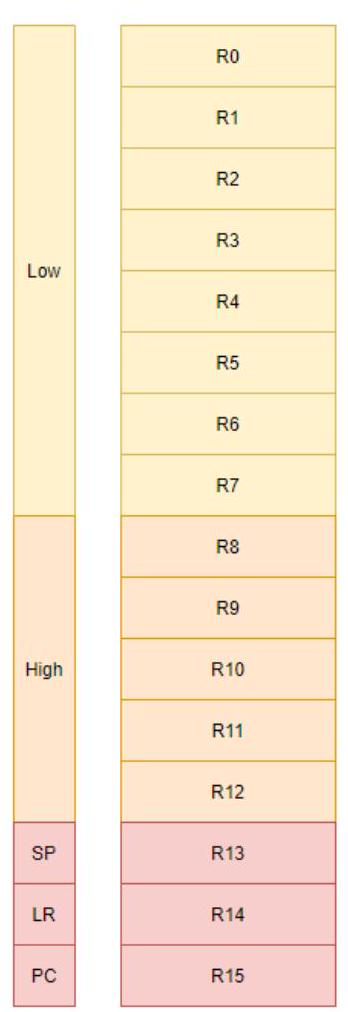
\includegraphics[width=0.35\linewidth, angle=90]{images/2024_12_29_79e6b22f503fb7b4f718g-02}

Main instruction types:
\begin{itemize}
  \item \textbf{Data Transfer}: Move, Load, Store operations
  \item \textbf{Data Processing}: Arithmetic, logical, shift operations
  \item \textbf{Control Flow}: Branch and function calls
\end{itemize}
\end{definition}

\begin{code}{Basic Assembly Program Structure}
Example of a simple assembly program:
\begin{lstlisting}[language=armasm, style=basesmol]
Label   Instr.  Operands   Comments
demoprg MOVS    R0,#0xA5   ;copy 0xA5 into R0
        MOVS    R1,#0x11   ;copy 0x11 into R1
        ADDS    R0,R0,R1   ;add R0 and R1, store in R0
\end{lstlisting}
\end{code}

\begin{concept}{Assembly Program Sections}\\
Program memory is organized in sections:

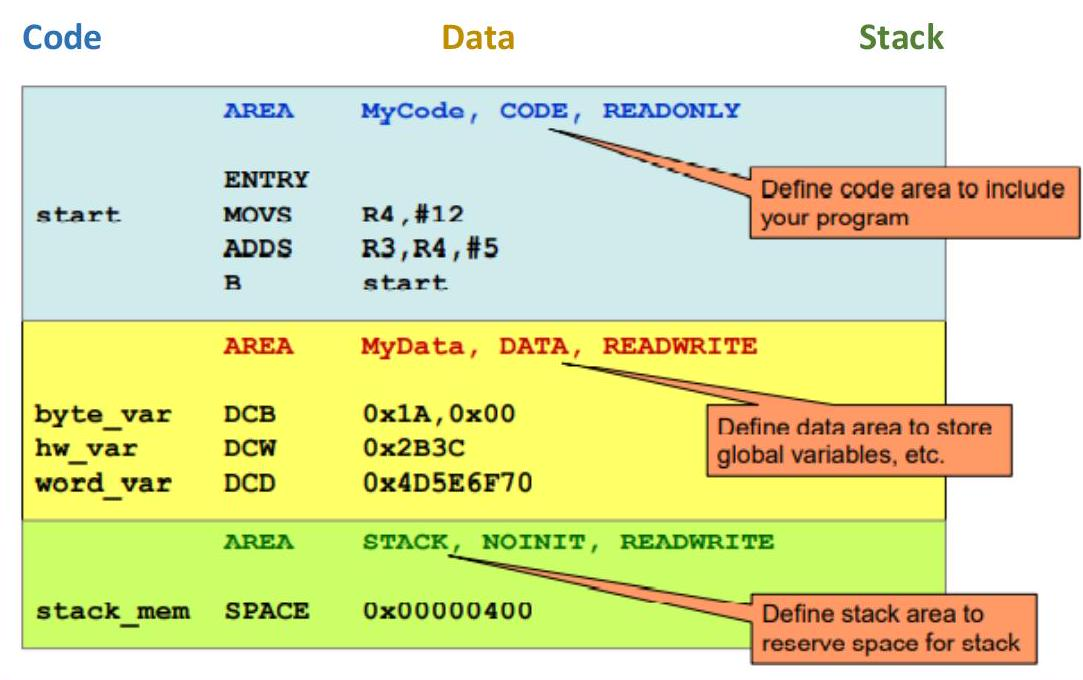
\includegraphics[width=\linewidth]{images/2024_12_29_79e6b22f503fb7b4f718g-02(1)}

\textbf{Directives for initialized data:}
\begin{itemize}
  \item \textbf{DCB}: Define Constant Byte (8-bit)
  \item \textbf{DCW}: Define Constant Half-Word (16-bit)
  \item \textbf{DCD}: Define Constant Word (32-bit)
\end{itemize}

\textbf{Directive for uninitialized data:}
\begin{itemize}
  \item \textbf{SPACE}: Reserve specified number of bytes
\end{itemize}
\end{concept}

\begin{code}{Data Definition}
Memory layout for different data types:
\begin{lstlisting}[language=armasm, style=basesmol]
var1    DCB     0x1A                ;single byte
var2    DCB     0x2B,0x3C,0x4D,0x5E ;byte array
var3    DCW     0x6F70,0x8192       ;half-words
var4    DCD     0xA3B4C5D6          ;word
data    SPACE   100                 ;reserve 100 bytes
\end{lstlisting}
\end{code}

\begin{KR}{Creating Assembly Programs}\\
Steps to create an assembly program:
\begin{enumerate}
  \item Define program sections (CODE, DATA)
  \item Declare any external symbols (IMPORT/EXPORT)
  \item Define initialized data using DCx directives
  \item Reserve uninitialized data using SPACE
  \item Write program code using proper instruction syntax
  \item End program with END directive
\end{enumerate}
\end{KR}

\section{Cortex-M Architecture}

\begin{concept}{Core Architecture Overview}\\
The ARM Cortex-M is a 32-bit processor architecture designed for embedded systems:
\begin{itemize}
  \item Load/store architecture
  \item 32-bit data path
  \item Thumb instruction set
  \item Hardware multiply and optional divide
  \item Harvard architecture variant (separate instruction and data buses)
  \item Designed for embedded applications:
    \begin{itemize}
      \item Low cost and power consumption
      \item Real-time capabilities
      \item Interrupt handling
      \item Debug support
    \end{itemize}
\end{itemize}
\end{concept}

\begin{definition}{Core Registers}\\
The Cortex-M has 16 core registers, each 32-bit wide:
\begin{itemize}
  \item \textbf{R0-R7}: Low registers - general purpose
    \begin{itemize}
      \item Used by most instructions
      \item Parameter passing in functions (R0-R3)
      \item Results returned in R0
    \end{itemize}
  \item \textbf{R8-R12}: High registers - general purpose
    \begin{itemize}
      \item Limited instruction support
      \item Often used for temporary storage
    \end{itemize}
  \item \textbf{R13 (SP)}: Stack Pointer
    \begin{itemize}
      \item Points to current stack position
      \item Must be word-aligned (multiple of 4)
    \end{itemize}
  \item \textbf{R14 (LR)}: Link Register
    \begin{itemize}
      \item Stores return address for function calls
      \item Can be saved to stack for nested calls
    \end{itemize}
  \item \textbf{R15 (PC)}: Program Counter
    \begin{itemize}
      \item Points to next instruction
      \item Auto-incremented during execution
    \end{itemize}
\end{itemize}
\end{definition}

\begin{definition}{ALU and Flags}\\
The Arithmetic Logic Unit (ALU) is 32-bit wide and supports:
\begin{itemize}
  \item Arithmetic operations:
    \begin{itemize}
      \item Addition (ADD, ADC)
      \item Subtraction (SUB, SBC)
      \item Multiplication (MUL)
      \item Division (Optional)
    \end{itemize}
  \item Logic operations:
    \begin{itemize}
      \item AND, ORR, EOR (XOR)
      \item BIC (Bit Clear)
      \item MVN (NOT)
    \end{itemize}
  \item Shift and rotate operations
  \item Compare operations
\end{itemize}

The Application Program Status Register (APSR) contains flags:
\begin{itemize}
  \item \textbf{N}: Set when result is negative (bit 31 = 1)
  \item \textbf{Z}: Set when result is zero
  \item \textbf{C}: Set on carry or borrow
  \item \textbf{V}: Set on signed overflow
\end{itemize}

Instruction suffix 'S' (e.g., ADDS) updates these flags.
\end{definition}

\begin{example2}{Flag Usage Examples}\\
After arithmetic operations with 'S' suffix:
\begin{lstlisting}[language=armasm, style=base]
    MOVS    R0, #0xFF    ; R0 = 255 (max unsigned 8-bit)
    ADDS    R0, #1       ; R0 = 0, Z=1, C=1 (overflow)
    
    MOVS    R0, #0x7F    ; R0 = 127 (max signed 8-bit)
    ADDS    R0, #1       ; R0 = 128, N=1, V=1 (signed overflow)
    
    MOVS    R0, #5
    SUBS    R0, #10      ; R0 = -5, N=1, C=0 (borrow)
\end{lstlisting}
\end{example2}